\documentclass[12pt]{article}
\usepackage{graphicx}
\usepackage{amsmath}
\usepackage{float}
\usepackage{pseudocode}
\addtolength{\textwidth}{1in}
\addtolength{\textheight}{1in}
\addtolength{\evensidemargin}{0.5in}
\addtolength{\oddsidemargin}{-0.5in}
\addtolength{\topmargin}{-0.5in}
\title{Generation of Minimal Well Formed Sudoku Puzzles}
\author{Taras Mychaskiw\\COSC 4P03 Project}
\date{April 22nd, 2014}

\begin{document}
\maketitle
    \begin{abstract}
    The purpose of this project was to generate minimal well formed sudoku puzzles. A well formed sudoku puzzle is one that has
    exactly one solution, and a minimal sudoku is one where you cannot remove any clue without making the puzzle not well formed.
    Several sudoku generating strategies are employed, as well as several solving strategies as the generation of sudoku puzzles
    inherently requires solving them and counting the number of solutions to them.
    \end{abstract}

    \thispagestyle{empty}
    \setcounter{tocdepth}{2}
    \tableofcontents
    %\cleardoublepage
    %\newpage
    \thispagestyle{empty}
    \mbox{}
    \clearpage
    \setcounter{page}{1}
    
    % COSC 4P03 Project
% sudoku generator
% Taras Mychaskiw

\section{Introduction}

\subsection{Terms}
Here are the terms and names that will be used in this paper.
\begin{center}\begin{tabular}{c||c}
    \hline
    $p$         &   the width of each box in the sudoku                             \\
    $q$         &   the height of each box in the sudoku                            \\
    $n$         &   the size of the entire sudoku grid, equal to $pq$               \\
    cell        &   each point which contains a value in the sudoku                 \\
    candidates  &   all the values that can lay in a cell                           \\
    unit        &   a set of cells where no two cells may share a value (eg a row)  \\
    peers       &   the set all of cells that a cell may not share a value with     \\
    formity     &   describes if a puzzle has none, one or many solutions           \\
    \hline
\end{tabular}\end{center}
%\end{Terms}

\subsection{Sudoku}
Sudoku is one of the most popular puzzle games of all time. A sudoku puzzle involves placing the numbers $1$ through $n$ in
a $n$x$n$ grid so that each row, each column and each $p$x$q$ box in the grid have each number exactly once. At the beginning of
a puzzle, several cells have values filled in, and the player's job is to fill in the rest of the grid. It is always
understood that every sudoku puzzle has exactly one solution to it. Figure~\ref{fig:sudoku} depicts a sample sudoku puzzle.
\begin{figure}[H]
    \centering
    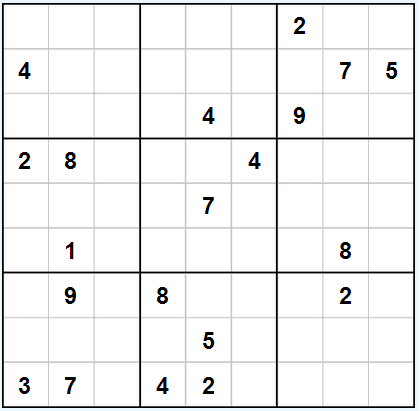
\includegraphics[scale=0.70]{sudoku.png}
    \caption{A standard $9$x$9$ sudoku puzzle.}
    \label{fig:sudoku}
\end{figure}

With the growing popularity of sudoku, many $9$x$9$ puzzles are required to feed the demand. Additionally, there is some demand
for larger or smaller sudoku puzzles (rather than $9$x$9$) for a greater or simpler challenge.
%\end{Sudoku}

%\end{Introduction}

    
    % COSC 4P03 Project
% sudoku generator
% Taras Mychaskiw

\section{Sudoku Solving Strategies}

Generating sudoku puzzles inherently requires being able to solve them. More specifically, the solver must be able to
check the formity of the sudoku puzzle and hopefully do it very quickly. Several solving strategies are used in the generation
in hopes that one will outperform the others and speed the generation process. Note that each of the algorithms described below
detail how to solve a puzzle, not how to get the formity of it. However, the algorithm to get the formity is only a slight
modification. For example, one could increment a counter keeping track of how many solutions there have been so far once
a solution is found instead of returning the solution right away.

\subsection{Backtracking}
Backtracking is the easiest solving strategy to understand. As the name suggests, it uses backtracking to solve the sudoku puzzle.
Algorithm~\ref{algo:backtrack} describes the basic idea below. Essentially, the algorithm goes through each cell in the sudoku and
tries assigning each possible value in a depth first search. If it finds a solution, the solved sudoku is returned right away. If
some candidate selection leads to an impossible to solve sudoku, the cell is cleared of it's value and the backtracking tries again
from the previous cell. To solve a sudoku puzzle using the backtracking algorithm, one would call $backtrack(sudoku, 0)$.
\begin{center}
\begin{pseudocode}[framebox]{backtrack}{sudoku, cell}
    \COMMENT{check if the sudoku is solved}                         \\
    \IF cell >= \CALL{getTotalCells}{sudoku} \THEN \RETURN {sudoku} \\
    \COMMENT{if there is already a value here, go to the next cell} \\
    \IF \CALL{hasValue}{sudoku, cell} \THEN
        \CALL{backtrack}{sudoku, cell + 1}                          \\
    \COMMENT{otherwise, try all candidates in depth first search}   \\
    \FOREACH cand \in \CALL{getCandidates}{sudoku, cell} \DO \BEGIN
        sudoku[cell] \GETS cand                                     \\
        board \GETS \CALL{backtrack}{sudoku, cell + 1}              \\
        \IF \CALL{isSolved}{board} \THEN \RETURN {board}            \\
    \END                                                            \\
    sudoku[cell] \GETS nothing                                      \\
    \RETURN {sudoku}~\COMMENT{the sudoku is not solved}
    \label{algo:backtrack}
\end{pseudocode}
\end{center}
%\end{Backtracking}

\subsection{Constraint Propagation}
Constraint propagation expands on the basic backtracking algorithm. It's more complex than backtracking, but solves sudoku puzzles
much faster on average. Constraint propagation tries to solve a sudoku puzzle in the same manner that a human would. Each cell on
the sudoku grid will contain a list of all the candidates to sit in that cell - similar to backtracking but they are used differently.
Two rules are employed in this solving method:
\begin{enumerate}
    \item if a cell only has one possible value, $eliminate$ the value from the cell's peers
    \item if a unit has only one possible cell for a value, $assign$ the value there
\end{enumerate}
These two rules continue to propagate, for example exercising rule 1 may trigger rule 2, which may trigger rule 1 and so on. Eventually,
either each cell in the entire puzzle will only have one candidate (in which case the puzzle is solved), or the propagation stops and the
puzzle is not yet solved. At that point, a version of backtracking will take place. A cell is selected, and one of it's candidate values
is simply assigned to the cell. If the assumption was incorrect, a backtrack would occur and a different value would be selected for the cell.
Which cell is selected differs from backtracking in that we choose the most constrained cell. That is, the cell with the fewest number of
candidates, but more than one candidate, is found and a value is assigned there. This helps to limit potential backtracking. The fewer number
of possibilities a cell has, the better chance that a random selection will end up being correct. 
To solve a particular sudoku puzzle, each of the cells that already contain values must be $assigned$, then call $search$. This implicitly means
that there is some pre-processing of a sudoku puzzle before solving the puzzle actually starts.
Algorithms~\ref{algo:assign} through~\ref{algo:clp} describe the flow of each function.
\begin{center}
\begin{pseudocode}[framebox]{assign}{cell, value}
    \GLOBAL{candidates} \\
    \FOR cand \in candidates[cell] - \{value\} \DO \CALL{eliminate}{cell, cand}
    \label{algo:assign}
\end{pseudocode}
\begin{pseudocode}[framebox]{eliminate}{cell, value}
    \GLOBAL{candidates, peers, units}   \\
    candidates[cell] \GETS candidates[cell] - \{value\}         \\
    \IF |candidates[cell]| = 1 \THEN \BEGIN
        v \GETS q \in candidates[cell]                          \\
        \FOR peer \in peers[cell] \DO \CALL{eliminate}{peer, v} \\
    \END                                                        \\
    
    \FOR unit \in units[cell] \DO \BEGIN
        otherCells \GETS \{~s~|~s \in unit, value \in candidates[s]~\}  \\
        \IF |otherCells| = 1 \THEN \BEGIN
            c \GETS q \in otherCells                                    \\
            \CALL{assign}{c, value}
        \END
    \END
    \label{algo:eliminate}
\end{pseudocode}
\begin{pseudocode}[framebox]{search}{ }
    \GLOBAL{candidates} \\
    \IF \exists~set = \emptyset~\forall set \in candidates \THEN \RETURN \FALSE     \\
    \IF |set| = 1, \forall set \in candidates \THEN \RETURN \TRUE                   \\
    cell \GETS c \text{ such that } |candidates[c]| > 1 \AND \text{is minimal}      \\
    \FOR cand \in candidates[cell] \DO \BEGIN
        \CALL{assign}{cell, cand}                   \\
        \IF \CALL{search}{} \THEN \RETURN {solved}
        \ELSE \CALL{revertAssign}{cell, cand}       \\
    \END                                            \\
    \RETURN \FALSE
    \label{algo:clp}
\end{pseudocode}
\end{center}
%\end{Constraint Propagation}

\subsection{Sudoku as an Exact Cover Problem}
    \subsubsection{Exact Cover}
    Before getting into how to solve sudoku puzzles by treating them as instances of the exact cover problem, we must know
    what the exact cover problem is. The exact cover problem is defined as:
    \begin{verse}
        given a collection $S$ of subsets of a set $X$, an \textit{exact cover} is a subcollection $S^*$ of $S$ such that each element
        in $X$ is contained in exactly one subset in $S^*$
    \end{verse}
    The exact cover problem is NP-Complete, proved by Karp in 1972\cite{npc}. One way to represent an exact cover problem is to use
    a matrix filled with boolean values. Each column of the matrix represent one element in $X$, and each row represents one of the
    subsets in $S$. Each of the boolean values in the matrix tell us if an element exists in the subset for that row. An example is
    detailed in the table below. Here, $X$ = $\{1,2,3,4,5,6\}$, and $S^*$ = $\{A,D,E\}$.
    \begin{center}\begin{tabular}{|c|c|c|c|c|c|c|}
        \hline
            &   1   &   2   &   3   &   4   &   5   &   6   \\  \hline
        $A$ &   0   &   1   &   0   &   0   &   0   &   0   \\  \hline
        $B$ &   0   &   0   &   1   &   1   &   1   &   0   \\  \hline
        $C$ &   0   &   1   &   0   &   0   &   0   &   0   \\  \hline
        $D$ &   0   &   0   &   1   &   0   &   1   &   1   \\  \hline
        $E$ &   1   &   0   &   0   &   1   &   0   &   0   \\
        \hline
    \end{tabular}\end{center}
    %\end{Exact Cover}
    
    \subsubsection{Algorithm X and Dancing Links}
    Donald Knuth introduced Algorithm X alongside Dancing Links in his 2000 paper\cite{dlx}. Algorithm X is defined as a non-deterministic
    backtracking algorithm that solves the exact cover problem when the problem is in the matrix form described above. The goal is to select
    a subset of rows of that matrix $A$ so that the true value appears only one in each column. Algorithm~\ref{algo:x} describes Algorithm X.
    \begin{center}\begin{pseudocode}[framebox]{algorithmX}{A}
        \IF A = \emptyset \THEN \RETURN \TRUE                           \\
        col \GETS \text{a column of }A                                  \\
        row \GETS \text{a row of }A\text{ such that }A[row][col] = 1    \\
        \text{include }row\text{ in the partial solution}               \\
        \FOR j \in \{~v~|~A[row][v] = 1~\} \DO \BEGIN
            \FOR i \in \{~w~|~A[w][j] = 1~\} \DO
                \text{remove row }i\text{from }A                        \\
            \text{remove column }j\text{from }A                         \\
        \END                                                            \\
        \text{repeat using the reduced matrix }A
        \label{algo:x}
    \end{pseudocode}\end{center}
    Dancing Links is an implementation of Algorithm X. At first glance of Algorithm X, it seems that much time would be wasted searching
    for $1$'s in the matrix $A$. Dancing Links provides a clever way to eliminate that search while also providing a very easy means for
    backtracking to occur. Dancing Links uses a quadruply linked list to represent the matrix, where each node in the list only contains
    the $1$'s in the matrix and are connected to the next $1$ in the matrix in direction. Additionally, there is a column header for each
    column, which each node in the column points to as well. Figure~\ref{fig:dlx} shows an example of the gigantic list that makes up Dancing Links.
    \begin{figure}[H]
        \centering
        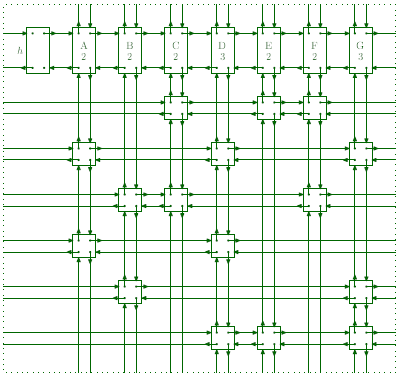
\includegraphics[scale=0.70]{dlx.png}
        \caption{An example matrix representation using Dancing Links.}
        \label{fig:dlx}
    \end{figure}
    The list removes the task of searching for $1$'s in the matrix, but as mentioned it's also very simple to remove columns from and
    re-add columns for backtracking. To remove a node from a column, for example, it requires:
    \begin{eqnarray}
        Node.left.right &=& Node.right  \nonumber   \\  
        Node.right.left &=& Node.left   \nonumber
    \end{eqnarray}
    And reinserting the node into the row requires:
    \begin{eqnarray}
        Node.left.right &=& Node    \nonumber   \\  
        Node.right.left &=& Node    \nonumber
    \end{eqnarray}
    Using Dancing Links as the implementation for Algorithm X, solving the exact cover problem becomes very fast.
    %\end{Algorithm X and Dancing Links}
    
    \subsubsection{Solving Sudoku as an Exact Cover Problem}
    Sudoku can be represented by an exact cover problem. Using the rules of sudoku, we can come up with the set $X$ and the collection
    of subsets $S$. If we think of each rule in sudoku as a column in the matrix $A$, then we can start to see how sudoku can be transformed
    into exact cover. Each of the rules must be satisfied exactly once, then the puzzle is solved. If we get an exact cover of the matrix where
    each of the column is a sudoku rule, then we solve that sudoku. The rules state that the values $1$ though $n$ must appear exact once in each
    row, column and box in the sudoku. Another implicit rule, but a very important one, is that each cell can only contain one value. This sums up
    to $4n^2$ total constraints that must be satisfied. Each of the $n$ rows, columns and boxes must contain $n$ values ($3n^2$), and each cell must
    contain a value which adds the final $n^2$. Each of these makes up a single element in $X$ - a single column of the matrix $A$.\\
    The collection of subsets in $n^3$ in size. For each cell, any value can sit in it. We can represent these by row, column and value triples,
    such as (row $1$, column $1$, value $1$), (row $1$, column $1$, value $2$) ... (row $n$, column $n$, value $n$). Each triple satisfies four
    constraints, the row-value, column-value and box-values pairs, and that the cell is occupied. If a cell contains a clue, then only one tuple
    appears in the matrix for that cell. Using this information we can construct the matrix $A$ then use Dancing Links to solve the puzzle.\\
    It should be noted that to use exact cover to solve sudoku, some pre-processing is required to create the matrix $A$. Afterwards, some
    post-processing is required to transform the matrix back into a sudoku puzzle.
    %\end{Solving Sudoku as an Exact Cover Problem}
%\end{Sudoku as an Exact Cover Problem}

%\end{Sudoku Solvung Strategies}

    
    % COSC 4P03 Project
% sudoku generator
% Taras Mychaskiw

\section{Sudoku Generation}

    \subsection{Top Down Generation}
    %\end{Top Down Generation}

    \subsection{Bottom Up Generation}
    %\end{Bottom Up Generation}

    \subsection{Deduction Generation}
    %\end{Deduction Generation}

%\end{Sudoku Generation}

    
    % COSC 4P03 Project
% sudoku generator
% Taras Mychaskiw

\section{Results}


%\end{Results}

    
    % COSC 4P03 Project
% sudoku generator
% Taras Mychaskiw

\section{Future Work}

An obvious extension of the work would be to devise more sudoku generation strategies, in order to produce sudoku puzzles with
fewer clues or produce very hard puzzles. Some additional ideas for generators that were never tested (due to time constraints)
are described below.

\begin{enumerate}
    \item starting from an empty sudoku, select the next clue to place in such a way that it limits the total amount of
    information given to the player, perhaps by maximizing the size of all the candidate sets for each remaining cell

    \item devise some difficulty ratings, and optimize them in the construction of the sudoku puzzle, perhaps a dynamic programming
    algorithm would be possible here to ensure the hardest puzzle in generated
\end{enumerate}

Solving sudoku puzzles does not need additional improvements (in \textit{my} opinion, at least). They are plenty fast, and when run
concurrently, one only reaps the benefits of each solver - the weaknesses of one solver are offset by the strengths of another.
However, if a faster sudoku solver is devised, it can only help the generation of puzzles.

%\end{Future Work}

\clearpage
\section{Conclusions}
All in all, the bottom up generation strategy was the most successful sudoku puzzle generator tested. It will occasionally produce an
effectively useless puzzle, but more often than not it outperforms the other generators in terms of the number of clues in the puzzles
created. It may take slightly more time, but it still created about $20$ sudoku puzzles per second on the computer running the tests.
In the future, one can remove the constraint propagation strategy entirely, and only run backtracking and exact cover solvers while
generating puzzles. This will ensure the unexpected benefits of backtracking and the raw speed of exact cover are both exploited.
%\end{Conclusions}

    
    % COSC 4P03 Project
% sudoku generator
% Taras Mychaskiw

\begin{thebibliography}{1}

\bibitem{slides}
Ross, B. "COSC 3P98 Lecture Slides" Brock University, Fall 2013

\bibitem{2p20text}
Fowles \& Cassiday "Analytical Mechanics, 7th Ed." Thomas Brooks/Cole, 2005

\bibitem{glui}
Paul Rademacher, "GLUI - A GLUT-Based User Interface Library" Version 2.0, 1999

\bibitem{3ds}
Damiano Vitulli, "3D Engine Programming Tutorials", Retreived December 2013 from
http://www.spacesimulator.net/wiki/

\bibitem{wpa}
World Pool-Billiard Association, "Table \& Equipment Specifications", Retreived December 2013 from
http://www.wpa-pool.com/

\end{thebibliography}


\end{document}
